\documentclass{article}

\usepackage{tikz}
\usepackage{subcaption}

\begin{document}
\pagestyle{empty}

\def\layersep{3.5cm}

\begin{figure}[!h]
	\begin{tikzpicture}[shorten >=1pt,->,draw=black!50, node distance=\layersep]
	   	\tikzstyle{every pin edge}=[<-,shorten <=1pt]
		\tikzstyle{neuron}=[circle,fill=black!25,minimum size=17pt,inner sep=0pt]
		\tikzstyle{input neuron}=[neuron, fill=green!50];
		\tikzstyle{output neuron}=[neuron, fill=red!50];
	   	\tikzstyle{hidden neuron}=[neuron, fill=blue!50];
		\tikzstyle{annot} = [text width=4em, text centered]

		% Draw the input layer nodes
		\node[input neuron, pin=left:$x_1$] (I-1) at (0,-1) {};
		\node[input neuron, pin=left:$x_2$] (I-2) at (0,-3) {};

		\path node[hidden neuron] (H-1) at (\layersep,-1 cm) {};
		\path node[hidden neuron] (H-2) at (\layersep,-3 cm) {};

	    	% Draw the output layer node %[yshift=0.5cm]
	    	\node[output neuron,pin={[pin edge={->}]right:y}, right of=H-1, yshift=-1.0cm] (O) {};

		% Connect every node in the input layer with every node in the
		% hidden layer.
		\path (I-1) edge node [above] {$w1$} (H-1) ;
		\path (I-1) edge node [pos=0.75, below, sloped] {$w3$} (H-2);
		\path (I-2) edge node [pos=0.75, above, sloped] {$w2$} (H-1);
		\path (I-2) edge node [below] {$w4$} (H-2);

		% Connect every node in the hidden layer with the output layer
		\path (H-1) edge node [above, sloped] {$w5$} (O);
		\path (H-2) edge node [below, sloped] {$w6$} (O);

		% Annotate the layers
		\node[annot,above of=H-1, node distance=1cm] (hl) {Hidden layer};
		\node[annot,left of=hl] {Input layer};
		\node[annot,right of=hl] {Output layer};
	\end{tikzpicture}
	\caption{The xor neural network.}
\end{figure}

\begin{figure}[!h]
	\centering
	\begin{subfigure}[b]{0.3\textwidth}
		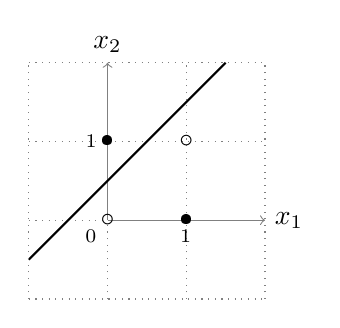
\begin{tikzpicture}[x=1cm,y=1cm]
			\draw[latex-latex, thin, draw=gray, ->] (0,0)--(2,0) node [right] {$x_1$};
			\draw[latex-latex, thin, draw=gray, ->] (0,0)--(0,2) node [above] {$x_2$}; 
			\draw[thick] (-1, -0.5)--(1.5, 2); 

			\draw [dotted, gray] (-1, -1) grid (2, 2);
			\node [black] at (0, 1) {\textbullet};
			\node [black] at (-0.2, 1) {$_1$};
			\node [black] at (1, 0) {\textbullet};
			\node [black] at (1, -0.2) {$_1$};
			\node [black] at (0, 0) {$\circ$} node [below left] {$_0$};
			\node [black] at (1, 1) {$\circ$};
		\end{tikzpicture}
		\caption{}
	\end{subfigure}
	\begin{subfigure}[b]{0.3\textwidth}
		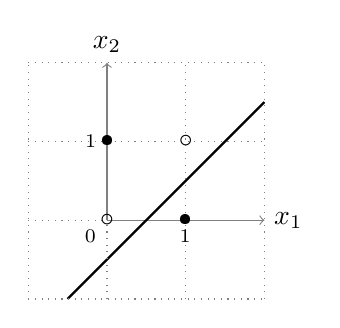
\begin{tikzpicture}[x=1cm,y=1cm]
			\draw[latex-latex, thin, draw=gray, ->] (0,0)--(2,0) node [right] {$x_1$};
			\draw[latex-latex, thin, draw=gray, ->] (0,0)--(0,2) node [above] {$x_2$}; 
			\draw[thick] (-0.5,-1)--(2, 1.5);

			\draw [dotted, gray] (-1, -1) grid (2, 2);
			\node [black] at (0, 1) {\textbullet};
			\node [black] at (-0.2, 1) {$_1$};
			\node [black] at (1, 0) {\textbullet};
			\node [black] at (1, -0.2) {$_1$};
			\node [black] at (0, 0) {$\circ$} node [below left] {$_0$};
			\node [black] at (1, 1) {$\circ$};
		\end{tikzpicture}
		\caption{}
	\end{subfigure}
	\begin{subfigure}[b]{0.3\textwidth}
		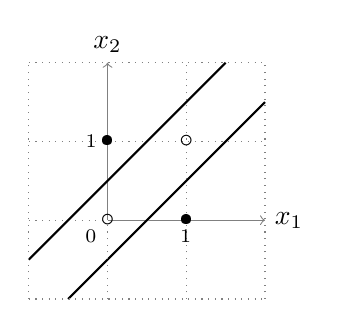
\begin{tikzpicture}[x=1cm,y=1cm]
			\draw[latex-latex, thin, draw=gray, ->] (0,0)--(2,0) node [right] {$x_1$};
			\draw[latex-latex, thin, draw=gray, ->] (0,0)--(0,2) node [above] {$x_2$}; 
			\draw[thick] (-1, -0.5)--(1.5, 2); 
			\draw[thick] (-0.5,-1)--(2, 1.5);

			\draw [dotted, gray] (-1, -1) grid (2, 2);
			\node [black] at (0, 1) {\textbullet};
			\node [black] at (-0.2, 1) {$_1$};
			\node [black] at (1, 0) {\textbullet};
			\node [black] at (1, -0.2) {$_1$};
			\node [black] at (0, 0) {$\circ$} node [below left] {$_0$};
			\node [black] at (1, 1) {$\circ$};
		\end{tikzpicture}
		\caption{}
	\end{subfigure}
	\caption{3 trials to seperate the classes. The filled circles are true cases and the empty circles are false cases.}
\end{figure}

\begin{figure}[!h]
	\centering
	\begin{tabular}{| l | c | r |}
		\hline
		$x_1$ & $x_2$ & $y$ \\ \hline
		0 & 0 & 0 \\ \hline
		0 & 1 & 1 \\ \hline
		1 & 0 & 1 \\ \hline
		1 & 1 & 1 \\ \hline
	\end{tabular}
	\caption{The truth table. When only one of the two input bits is true, the output bit should be true.}
\end{figure}	

\end{document}

